\section{Method: TissuePMHC Human Model}

\subsection{Architecture and Task-specific Prediction}

The TissuePMHC human model is designed for the human tissue--HLA benchmark, where tasks share peptide-level regularities but also exhibit allele-specific motifs and tissue-dependent differences. The model therefore uses two complementary branches. A global auxiliary branch is trained jointly across all tissue--HLA tasks and is regularized by tissue and HLA classification objectives. An HLA-specific branch trains one grouped model for each HLA allele and shares representations only among tissues associated with that allele. Both branches use the same position-preserving multi-kernel peptide encoder and task-specific binary prediction heads. Their output probabilities are converted to percentile ranks within each task, averaged with fixed equal weights, and finally averaged across independently trained random seeds.

This design separates three forms of statistical sharing. The convolutional encoder learns local sequence patterns that can recur across tasks; task-specific heads preserve different decision boundaries for individual tissue--HLA combinations; and the two branches impose global versus allele-restricted sharing structures. The architecture is not intended to predict an unseen task because its final prediction depends on a head associated with a tissue--HLA combination represented during fitting.

\begin{figure}[tbp]
\centering
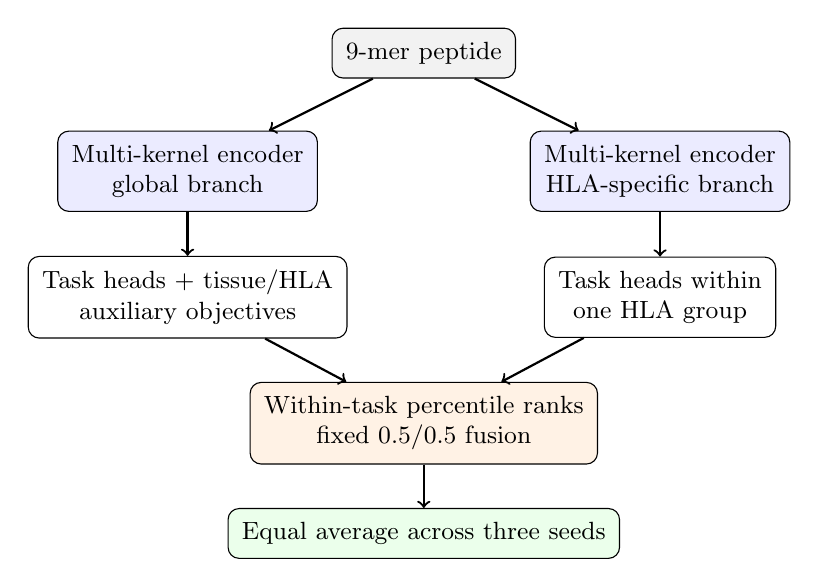
\begin{tikzpicture}[
    box/.style={draw,rounded corners,align=center,inner sep=5pt,font=\small},
    arr/.style={->,thick}
]
\node[box,fill=gray!10] (pep) at (0,0) {9-mer peptide};
\node[box,fill=blue!8] (encg) at (-3,-1.5) {Multi-kernel encoder\\global branch};
\node[box,fill=blue!8] (ench) at (3,-1.5) {Multi-kernel encoder\\HLA-specific branch};
\node[box] (global) at (-3,-3.1) {Task heads + tissue/HLA\\auxiliary objectives};
\node[box] (hla) at (3,-3.1) {Task heads within\\one HLA group};
\node[box,fill=orange!10] (fusion) at (0,-4.7) {Within-task percentile ranks\\fixed 0.5/0.5 fusion};
\node[box,fill=green!8] (seed) at (0,-6.1) {Equal average across three seeds};
\draw[arr] (pep) -- (encg);
\draw[arr] (pep) -- (ench);
\draw[arr] (encg) -- (global);
\draw[arr] (ench) -- (hla);
\draw[arr] (global) -- (fusion);
\draw[arr] (hla) -- (fusion);
\draw[arr] (fusion) -- (seed);
\end{tikzpicture}
\caption{TissuePMHC human-model architecture. Auxiliary tissue/HLA classifiers are training-only regularizers; inference uses the two task-head scores, within-task rank fusion, and seed averaging.}
\label{fig:tissuepmhc-architecture}
\end{figure}

Let \(h_i\) denote the encoded representation of peptide \(p_i\), and let \(\tau_i\) be its tissue--HLA task. Each branch maintains a separate linear head for every task available to that branch. The main-task logit is
\[
z_i=g_{\tau_i}(h_i),
\]
and the associated presentation-preference probability is
\[
q_i=\sigma(z_i),
\]
where \(\sigma\) is the logistic sigmoid. During a mini-batch update, examples are routed to the corresponding task heads while the encoder parameters are shared according to the branch definition. The main-task loss is binary cross-entropy with logits:
\[
\mathcal{L}_{\mathrm{BCE}}
=
-\frac{1}{B}
\sum_{i=1}^{B}
\left[
y_i\log q_i+(1-y_i)\log(1-q_i)
\right].
\]
Although every benchmark pair contains one positive and one pseudo-negative row, the model processes rows independently and does not use pair identifiers in the forward pass or training objective.

\subsection{Position-preserving Multi-kernel Encoder}

For a 9-mer peptide \(p=(a_1,\ldots,a_9)\), each residue is mapped to a learned embedding of dimension \(d=16\). A learned positional embedding is added at every sequence position. The resulting input matrix is
\[
X=E(p)+P \in \mathbb{R}^{9\times d},
\]
where \(E(p)\) contains residue embeddings and \(P\) is a trainable \(9\times d\) positional representation shared across peptides. Positional embeddings make the same amino acid distinguishable across locations, which is important because MHC-I anchor and auxiliary positions are not interchangeable.

The model operates only on standard 9-mer peptides in the present benchmark. No tissue transcriptomics, proteomics, parent-protein sequence, flanking sequence, or external binding score is supplied as input. Tissue and HLA information enter through task identities, prediction heads, sharing structure, and training-time auxiliary targets rather than through additional omics measurements.

Following multi-width convolutional sequence encoders \cite{kim2014cnn}, we apply one-dimensional convolutions with kernel sizes
\[
\mathcal{K}=\{2,3,5\}.
\]
For each \(k\in\mathcal{K}\), the input is transposed to a channels-first representation and processed as
\[
H_k
=
\operatorname{ReLU}
\left(
\operatorname{Conv1D}_{k}(X)
\right).
\]
Each convolution produces 32 channels. Padding is chosen to retain local context at peptide boundaries. For even-sized kernels, symmetric padding produces one additional position, so the implementation deterministically crops the output back to the first nine positions. Consequently, every branch yields
\[
H_k\in\mathbb{R}^{9\times 32}.
\]

The three feature maps are concatenated along the channel dimension while preserving their sequence positions. Rather than applying global max or average pooling, the model flattens all nine position-specific slots:
\[
v
=
\operatorname{Flatten}
\left[
H_2;H_3;H_5
\right]
\in\mathbb{R}^{9\cdot32\cdot3}.
\]
The flattened vector is passed through a two-layer multilayer perceptron,
\[
h
=
\operatorname{MLP}(v)
\in\mathbb{R}^{128},
\]
where each hidden layer has 128 units and a ReLU activation, and dropout with probability 0.2 is applied after the first hidden activation. Flattening is deliberate: it allows identical local patterns at different peptide positions to contribute differently to the final representation. The multi-kernel construction should be interpreted as a position-aware peptide encoder tailored to the fixed-length benchmark, rather than as a claim that convolution itself is novel.

\subsection{Global and HLA-specific Sharing}

The global branch uses a single encoder shared across all human tasks and one main prediction head per tissue--HLA combination. Two auxiliary linear classifiers operate on the same encoded representation \(h_i\): one predicts the tissue label and the other predicts the HLA label. If \(c_i^{(t)}\) and \(c_i^{(m)}\) denote the tissue and HLA categories, respectively, the branch objective is
\[
\mathcal{L}_{\mathrm{global}}
=
\mathcal{L}_{\mathrm{BCE}}
+
\lambda_t
\mathcal{L}_{\mathrm{CE}}
\left(
\widehat{c}^{(t)},c^{(t)}
\right)
+
\lambda_m
\mathcal{L}_{\mathrm{CE}}
\left(
\widehat{c}^{(m)},c^{(m)}
\right),
\]
with fixed weights
\[
\lambda_t=\lambda_m=0.1.
\]
The auxiliary classifiers are used only during training. They encourage the shared peptide representation to retain information associated with tissue and HLA groupings, but they do not constitute tissue-specific molecular inputs and are not consulted when generating final scores. Their role is therefore regularization of the representation rather than independent evidence at inference time.

The HLA-specific branch restricts parameter sharing to tasks with the same allele. For each HLA allele \(m\), we define
\[
\mathcal{T}_m
=
\{(t,m)\in\mathcal{T}\}.
\]
A separate encoder is trained on the rows belonging to \(\mathcal{T}_m\), and each tissue--HLA task in the group receives its own linear head. The objective for allele \(m\) is
\[
\mathcal{L}_{m}
=
\frac{1}{|\mathcal{D}_m|}
\sum_{i\in\mathcal{D}_m}
\mathcal{L}_{\mathrm{BCE}}
\left(
g^{(m)}_{\tau_i}(h_i^{(m)}),y_i
\right).
\]
No tissue or HLA auxiliary classifier is used in this branch. Because all examples within a grouped model already share the allele, the branch concentrates its capacity on allele-specific peptide patterns and variation among tissues under the same HLA restriction. It complements the global branch: global sharing can stabilize long-tailed tasks, whereas HLA-restricted sharing can preserve motif structure that unrestricted pooling may blur.

\subsection{Fixed Task-wise Rank Fusion}

The global and HLA-specific branches produce probabilities whose numerical scales may differ because the branches use different sharing structures and are trained independently. We therefore normalize predictions within each task before combining them. For task \(\tau\), let \(q_{g,i}\) and \(q_{h,i}\) be the global and HLA-specific branch probabilities for row \(i\). We compute average-tie percentile ranks
\[
r_{g,i}
=
\operatorname{PercentileRank}_{\tau}(q_{g,i}),
\qquad
r_{h,i}
=
\operatorname{PercentileRank}_{\tau}(q_{h,i}).
\]
The fused prediction for one seed is
\[
s_i^{(b)}
=
\frac{r_{g,i}+r_{h,i}}{2}.
\]
Both branch weights are fixed at 0.5. They are not selected on the test set or adapted task by task. Rank fusion preserves the within-task ordering information most relevant to AUROC and reduces sensitivity to branch-specific calibration. It does not produce an absolute presentation probability and should not be interpreted as a calibrated risk score. In the standard fixed test, the percentile-rank reference set is the complete evaluation batch for the corresponding tissue--HLA task. In out-of-fold experiments, it is the rows of that task in the current outer held-out fold; ranks are not estimated from the fitting partition or from a separate calibration set. The reported fusion is therefore a batch-level ranking procedure: adding or removing candidates can change their ranks, and an isolated candidate has no standalone rank-fused score. Prospective use would require either a prespecified candidate batch or a frozen reference distribution for mapping branch probabilities; this study evaluates only the former batch-ranking setting.

\subsection{Multi-seed Ensemble and Scope}

For each seed \(b\in\{1,\ldots,B\}\), both branches are trained and fused as above. Following the deep-ensemble principle \cite{lakshminarayanan2017deep}, the final score averages the per-seed fused ranks:
\[
s_{i,\mathrm{final}}
=
\frac{1}{B}
\sum_{b=1}^{B}
s_i^{(b)},
\qquad B=3.
\]
Thus, branch probabilities are first converted to within-task ranks and fused inside each seed; the resulting fused scores are then averaged across seeds. This order is fixed across standard and peptide-disjoint experiments.

The ensemble point estimate must not be confused with training stability. Averaging three members produces a single prediction vector and therefore cannot by itself demonstrate zero random variation. We separately report the distribution of the three single-seed results, together with the ensemble result, so that performance gains from variance reduction remain distinguishable from between-seed uncertainty.

\subsection{Mouse Factorized MMoE}

The mouse benchmark uses a separately trained task-balanced Factorized MMoE. Each residue has a 16-dimensional embedding; the flattened 9-mer is projected to a 128-dimensional peptide vector by a ReLU layer with dropout 0.2. Three experts apply 128-to-64 and 64-to-64 ReLU layers, with dropout after the first layer. The gate combines the peptide vector with 16-dimensional tissue and H2 embeddings, then applies a 64-unit ReLU layer and a three-way softmax. The mixture feeds 24 task-specific linear heads. The model has 68,475 trainable parameters.

Training uses task-balanced mini-batches: every update samples 16 rows with replacement from each of the 24 tasks, and the objective gives equal weight to the 24 task-wise binary cross-entropies. A gate-entropy term with coefficient 0.01 is subtracted from this mean loss to discourage premature routing collapse. AdamW, the 25-epoch budget, learning rate \(10^{-3}\), weight decay \(10^{-4}\), and gradient-norm cap of 1.0 follow the common training protocol. The standard and peptide-disjoint mouse results average predicted probabilities with equal weight across seeds 20260704--20260708; neither seed subsets nor ensemble weights are selected from the fixed test or strict OOF predictions. The H2-Kk adapter baseline retains this backbone and modifies only H2-Kk rows: for the 128-dimensional peptide representation \(h\), it adds \(A(h)=W_2\operatorname{ReLU}(W_1h)\), where \(W_1\) maps 128 to 16 dimensions and \(W_2\) maps 16 back to 128; other H2 groups use \(h\) unchanged. H2-Kk was predeclared from the completed backbone diagnosis, and the adapter was evaluated by three-fold pair-grouped OOF with seeds 20260704--20260706, without access to the fixed test.

The TissuePMHC human model and the frozen mouse Factorized MMoE are species-specific methods; no parameter is transferred between them. The comparison tests benchmark-level reproducibility, not a shared representation or biological mechanism.
